\section{Evaluation}
\subsection{Storage I/O }
Storage I/O is a key component for most scientific HPC applications. For example, large-scale simulations often need to first load large datasets before computation and frequently record the state during computation and once the simulation has concluded. Later, these results may be used for other simulations or for analytics. I/O performance plays an important role for the overall performance of an HPC application. In this section, we conduct experimental evaluation of the storage I/O performance of \texttt{BEE-VM} on an HPC system. In particular, we test and compare the performance of our two storage designs and native performance. To accurately evaluate storage I/O performance, we use the benchmark tool IOR \cite{IOR}. We simulate a situation where there is one process per node and each process writes and then reads 1GB of a datafile stored in the shared storage directory using MPI-IO functions. To avoid inaccurate results caused by caching, each process only reads files that are produced by another process on a different node. 

\begin{figure}[h]
    \centering
    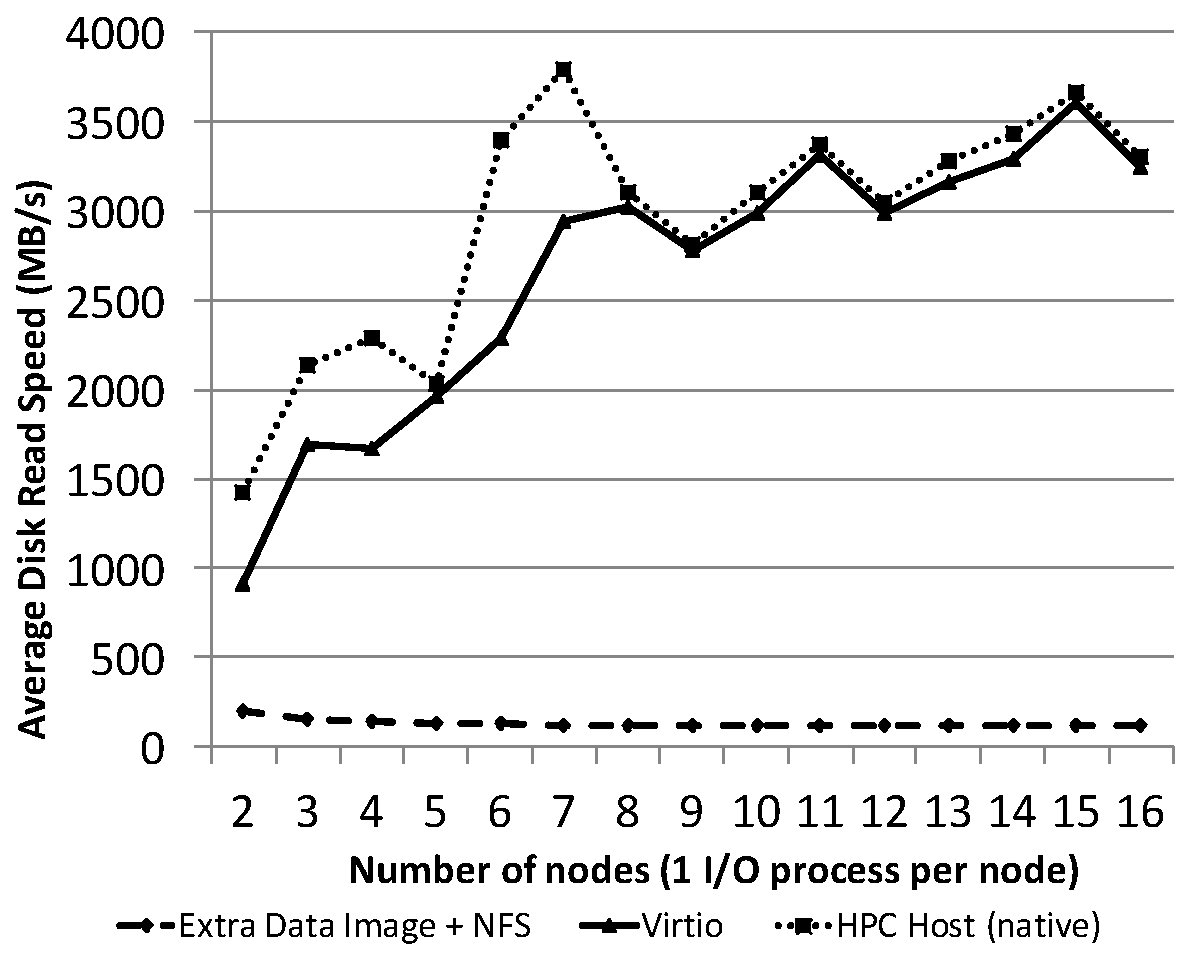
\includegraphics[width=0.5\textwidth]{figures/io-read-seq-test.pdf}
    \caption{Storage I/O read test comparison on different storage designs of BEE-VM. Results show that Virtio outperforms \texttt{Data image + NFS} with similar performance to native.}
    \label{io-test-read}
    %\vspace*{-2em}
\end{figure}

\begin{figure}[h]
    \centering
    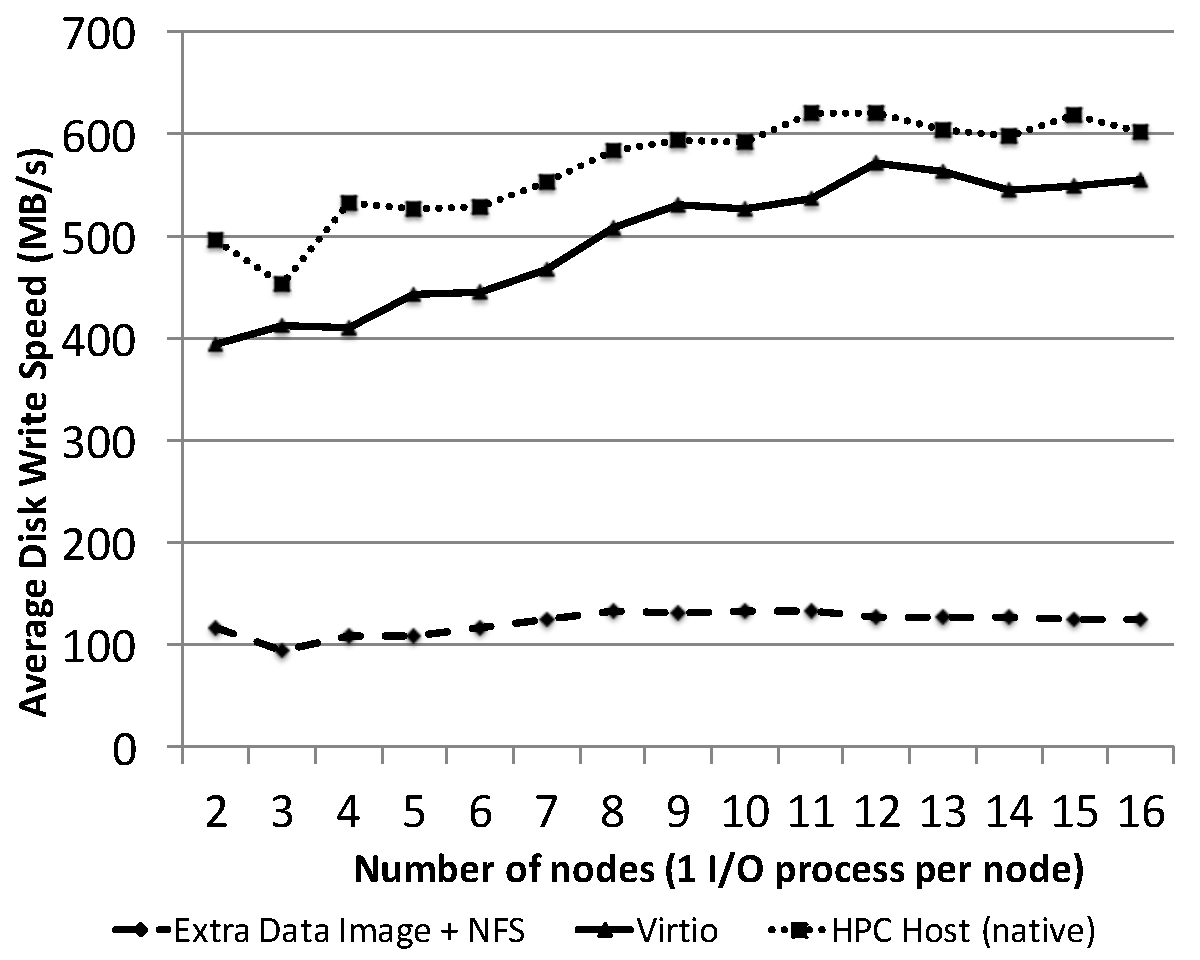
\includegraphics[width=0.5\textwidth]{figures/io-write-seq-test.pdf}
    \caption{Storage I/O write test comparison on different storage designs of BEE-VM. Results show that Virtio can achieve 90\% of the performance of native.}
    \label{io-test-write}
    %\vspace*{-1em}
\end{figure}

The result is shown in \textbf{Fig. \ref{io-test-read}} for read performance and \textbf{Fig. \ref{io-test-write}} for write performance of our two different storage solutions using different numbers of nodes. \texttt{Data image + NFS} solution does not rely on host file sharing capabilities. When using \texttt{Data image + NFS} design, except the master node which directly mounts the data image though the hypervisor driver, other worker nodes all mount the shared directory through NFS, which depends on the network between master and workers. Since all I/O requests must go through the master node, the network performance of the master node becomes the upper bound of storage I/O performance. As the number of worker nodes increases, the master node becomes a hot spot, which limits the overall I/O performance.  As shown in \textbf{Fig. \ref{io-test-read}} and \textbf{\ref{io-test-write}}, the read and write speed of this solution are always near 120-130 MB/s no matter how many nodes participate. \texttt{Virtio} design utilizes the file system mapping feature of the hypervisor. All storage I/O requests are sent to and processed by the hypervisor driver. It offers better performance and saves all user space network for MPI communication. As we can see in \textbf{Fig. \ref{io-test-read}} and \textbf{\ref{io-test-write}}, this design can achieve almost the same native I/O read performance and 90\% native I/O write performance on an HPC system. 

\subsection{Network through IB}
In this section, we show that network performance result comparison of BEE using the Infiniband (IB) on Chameleon Cloud. The BEE-Chameleon can actually be deployed on any HPC and cloud environment that is equipped with IB and Single Root Input/Output Virtualization (SR-IOV). The target system may or may not have privileged access, so we implemented BEE-Chameleon with two configurations: Docker only (for systems with privileged access) and Docker + KVM (for systems without privileged access). \textbf{Fig. \ref{ib-bandiwdth}, \ref{ib-latency}} show the point-to-point (P2P) network performance. MPI communication function calls between two nodes (one process per node) were used to test the average bandwidth and latency when transferring different message sizes. In \textbf{Fig. \ref{ib-scaliability}}, we also show the result of network scalability test using MPI all-to-all function call with different message sizes. Limited by the Chameleon Cloud reservation policy, we can only allocate up to 16 nodes. It can be seen that our BEE-Chameleon can provide similar network bandwidth, latency, and scalability compare to the baremetal. It also shows promising trends on larger clusters. Similar results have been seen in \cite{zhang2016performance}. Note that the Docker container is slightly better than baremetal in some cases due to the tuning difference under the test scenario.  

\begin{figure}[h]
    \centering
    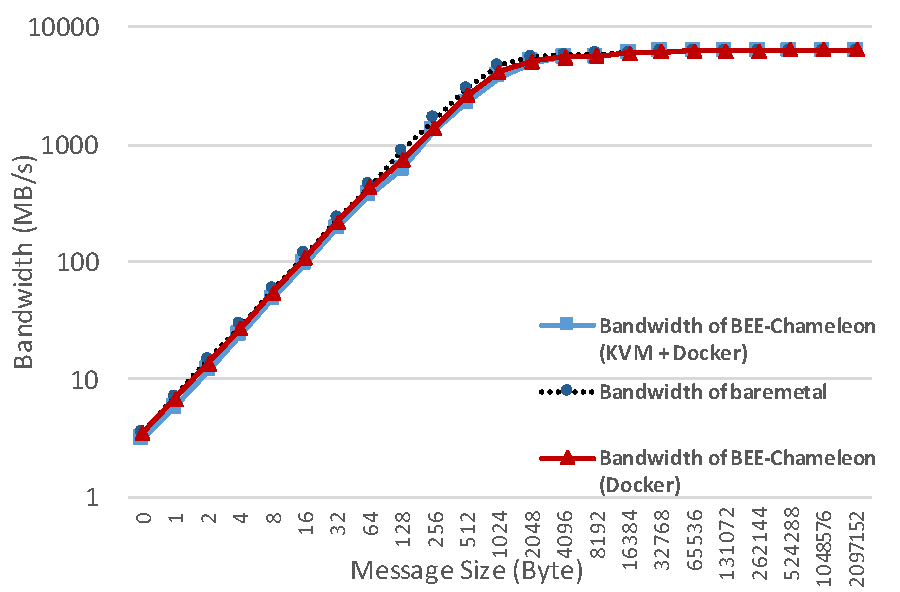
\includegraphics[width=0.5\textwidth]{figures/ib-bandwidth.pdf}
    \caption{IB bandwidth comparison}
    \label{ib-bandiwdth}
    %\vspace*{-2em}
\end{figure}

\begin{figure}[h]
    \centering
    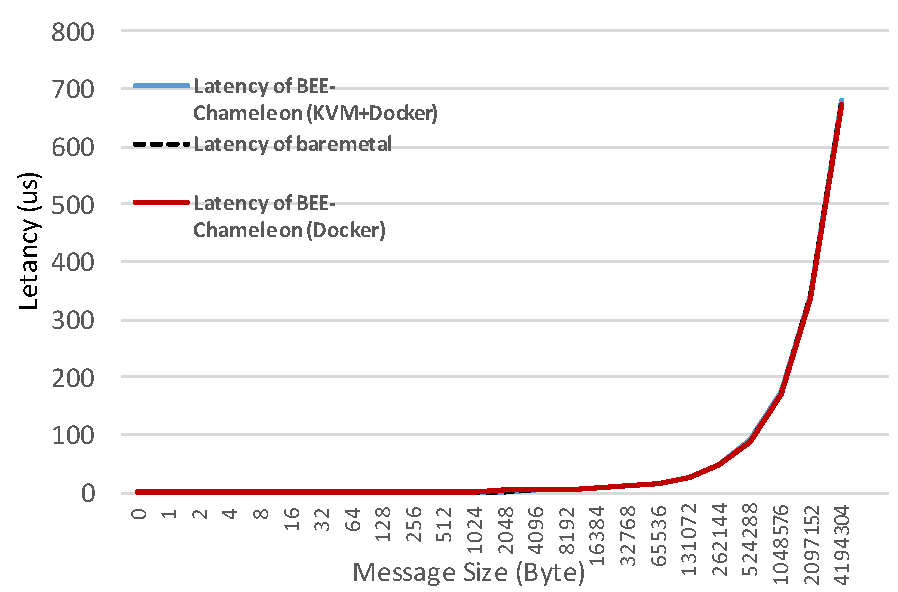
\includegraphics[width=0.5\textwidth]{figures/ib-latency.pdf}
    \caption{IB latency comparison}
    \label{ib-latency}
    %\vspace*{-2em}
\end{figure}

\begin{figure}[h]
    \centering
    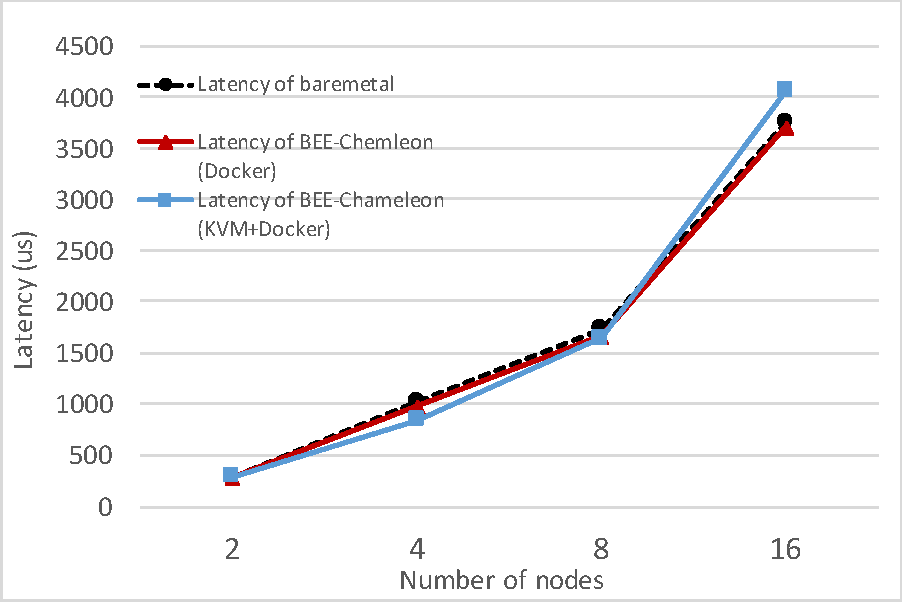
\includegraphics[width=0.5\textwidth]{figures/ib-scaliability.pdf}
    \caption{IB scalability comparison}
    \label{ib-scaliability}
    %\vspace*{-2em}
\end{figure}

\subsection{Performance Degradation}
Computing capability is another factor that needs to be considered for running HPC applications. In this section, we compare the computing performance of an HPC host with KVM-enabled virtual machines and our virtualized \texttt{BEE-VM} environment. We also compared the performance on AWS and virtualized \texttt{BEE-AWS}. This test is designed to show both the computing power of virtualized CPUs and memory access performance.  We run CoMD\cite{comd}, an HPC proxy application, on a single multicore computing node with KVM enabled.

\begin{figure}[h]
    \centering
    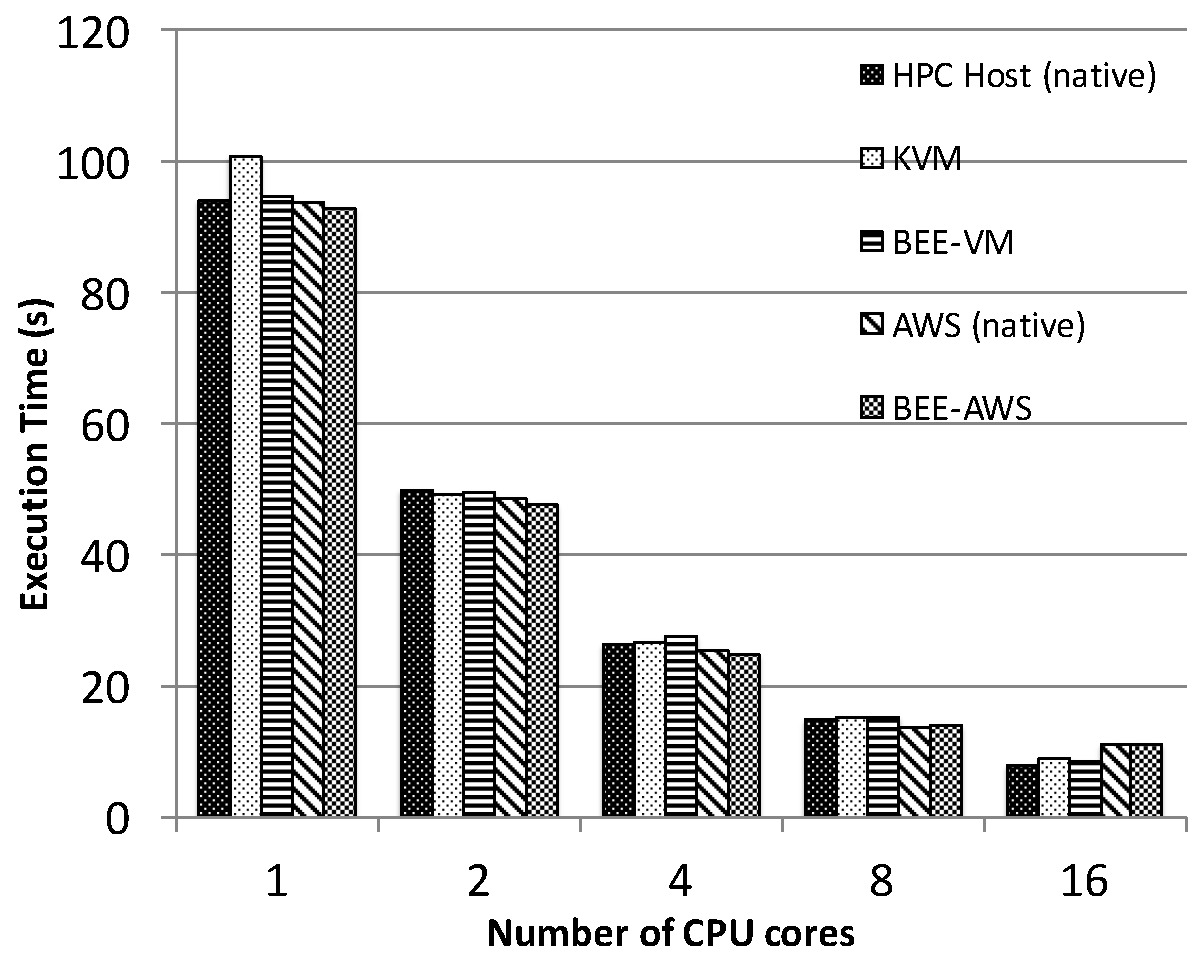
\includegraphics[width=0.5\textwidth]{figures/lu.pdf}
    \caption{Computing performance comparison between HPC host, KVM, BEE-VM, AWS, and BEE-AWS. Both BEE-VM and BEE-AWS virtualized environments provide comparable performance to native performance of HPC and AWS on a single node.}
    \label{comp-test}
    %\vspace*{-2em}
\end{figure}
 As shown in \textbf{Fig. \ref{comp-test}}, although we bring two layers of virtualization for \texttt{BEE-VM} and \texttt{BEE-AWS}, it only adds slight overhead (approximately 9\%) to the application. It also performs well in multicore environments. The overhead percentage almost stays constant for the different number of CPU cores used. This shows that our \texttt{BEE} framework using \texttt{BEE-VM} and \texttt{BEE-AWS} can achieve near native computing capabilities. 
